\documentclass[10pt,
	american,
	sections numbered,
	usenames,
	xcolor=dvipsnames,
	aspectratio=169,
]{beamer}

\mode<presentation>
\usepackage{kotex}
\usepackage{babel}
\usepackage[babel]{microtype}
\usepackage[babel]{csquotes}
\usepackage[american]{isodate}

\usepackage[T1]{fontenc}
\usepackage{FiraMono}

\usetheme[progressbar=frametitle]{metropolis}

%%% GRAPHICS %%%
\usepackage{graphicx}
\usepackage{pgfplots}
\usepackage{tikz}
\newcommand*\circled[1]{\tikz[baseline=(char.base)]{
            \node[shape=circle,draw,inner sep=1pt] (char) {#1};}}

%%% MATH & SCIENCE %%%
\usepackage{amsmath}
\usepackage{amssymb}
\usepackage{amsfonts}
\usepackage{amsthm}
\usepackage{siunitx}
\usepackage{bm}
\usepackage{dsfont}
\usepackage{mathtools}

%%% FLOATS %%%
\usepackage{booktabs}
\usepackage{tabularx}
\usepackage{tabu}

%\usepackage{biblatex}
%\bibliography{literature.bib}

\usepackage{tabu}

\long\def\term#1{%
 \ifmmode\ensuremath{\color{MidnightBlue}\boldmath#1}%
 \else
 {\bfseries\color{MidnightBlue}\boldmath#1}%
 \fi%
}

\def\myem#1{
 \ifmmode\ensuremath{\color{BrickRed}\boldmath#1}%
 \else
 {\sffamily\bfseries\color{BrickRed}\boldmath#1}%
 \fi
}

\def\mybf#1{
\ifmmode\ensuremath{\color{RoyalBlue}\boldmath#1}%
\else
{\sffamily\bfseries\color{RoyalBlue}\boldmath#1}%
\fi
}

\def\mybff#1{
 \ifmmode\ensuremath{\color{PineGreen}\hspace*{-12pt}\boldmath#1}%
 \else
 {\sffamily\bfseries\color{PineGreen}\hspace*{-12pt}\boldmath#1}%
 \fi
}

\def\mybfff#1{
 \ifmmode\ensuremath{\color{Violet}\boldmath#1}%
 \else
 {\sffamily\bfseries\color{Violet}\boldmath#1}%
 \fi
}

\newcommand*{\mypf}{{\par\color{bgcolorAlt!90!fgcolor}\mybf{\textsc{Proof}}\hrulefill\par}}


\graphicspath{{figs/}}  

% DESIGN COLORS
\definecolor{accent}{HTML}{7EBDC2} % accent color
\definecolor{bgcolor}{HTML}{FCFCFF} % background color
\definecolor{bgcolorAlt}{HTML}{ECF1FC} % alternative background color
\definecolor{fgcolor}{HTML}{222244} % foreground/text color

%
\setbeamercolor{normal text}{%
	fg=fgcolor,
	bg=bgcolor,
}
\setbeamercolor{alerted text}{%
	fg=accent,
}
\setbeamercolor{palette primary}{%
	use=normal text,
	fg=normal text.fg,
	bg=bgcolorAlt,%normal text.bg
}

\setbeamercolor{block title}{
	bg=bgcolorAlt,
}
\setbeamercolor{block body}{
	bg=bgcolorAlt,
}
\setbeamercolor{block title alerted}{%
	use={palette primary, alerted text},
	fg=palette primary.bg,
	bg=alerted text.fg
}
\setbeamercolor{block title example}{%
	use={block title, alerted text},
	bg=block title.bg,
	fg=alerted text.fg
}
%

\pgfplotsset{legend style={fill=bgcolor,draw=fgcolor}}

% PLOT COLORS
%% Paul Tol High Contrast
\definecolor{plot0}{HTML}{004488}
\definecolor{plot1}{HTML}{DDAA33}
\definecolor{plot2}{HTML}{BB5566}
\definecolor{plot3}{HTML}{000000}
\definecolor{plot4}{HTML}{AAAAAA}

%% Paul Tol Vibrant
%\definecolor{plot0}{HTML}{EE7733}
%\definecolor{plot1}{HTML}{0077BB}
%\definecolor{plot2}{HTML}{33BBEE}
%\definecolor{plot3}{HTML}{EE3377}
%\definecolor{plot4}{HTML}{CC3311}
%\definecolor{plot5}{HTML}{009988}
%\definecolor{plot6}{HTML}{BBBBBB}

\pgfplotscreateplotcyclelist{lineplot cycle}{ %
	{plot0, mark=*, thick, mark options=solid},
	{plot1, mark=triangle*, thick, mark options=solid},
	{plot2, mark=square*, thick, mark options=solid},
	{plot3, mark=diamond*, thick, mark options=solid},
	{plot4, mark=pentagon*, thick, mark options=solid},
}
%\renewcommand*{\bibfont}{\scriptsize}
\setbeamerfont{block body reference}{size=\scriptsize}
\setbeamerfont{block title reference}{size=\scriptsize}

\setbeamerfont{description item}{series=\mdseries}
\setbeamerfont{alerted text}{series=\bfseries\boldmath}


\setbeamertemplate{title page}{
\begin{minipage}[b][\textheight]{\textwidth}
	\ifx\inserttitlegraphic\@empty\else\usebeamertemplate*{title graphic}\fi
	\vfill%
	\ifx\inserttitle\@empty\else\usebeamertemplate*{title}\fi

	\usebeamertemplate*{title separator}
	\ifx\insertsubtitle\@empty\else\usebeamertemplate*{subtitle}\fi
	\ifx\beamer@shortauthor\@empty\else\usebeamertemplate*{author}\fi
	\ifx\insertdate\@empty\else\usebeamertemplate*{date}\fi
	\ifx\insertinstitute\@empty\else\usebeamertemplate*{institute}\fi
	\vfil
	\vspace*{1mm}
\end{minipage}
}
\newcommand*{\seprule}{{\par\color{bgcolorAlt!90!fgcolor}\hrulefill\par\vspace*{1ex plus 0pt minus .5ex}}}

% Mathematical Writing
\DeclarePairedDelimiter{\abs}{\vert}{\vert}
\DeclarePairedDelimiter{\norm}{\Vert}{\Vert}
\DeclarePairedDelimiter{\ceil}{\lceil}{\rceil}
\DeclarePairedDelimiter{\floor}{\lfloor}{\rfloor}

\newcommand*{\inv}[1]{\ensuremath{#1^{-1}}}
\newcommand*{\positive}[1]{\ensuremath{\left[#1\right]^{+}}}

\newcommand*{\diff}{\ensuremath{\mathrm{d}}}
\newcommand*{\imag}{\ensuremath{\mathrm{j}}}
\newcommand*{\e}{\ensuremath{\mathrm{e}}}

\DeclareMathOperator*{\argmax}{arg\,max}
\DeclareMathOperator*{\argmin}{arg\,min}

%% change these to \mathbb, if you do not want to use the dsfont package
\newcommand*{\reals}{\ensuremath{\mathds{R}}} 
\newcommand*{\complexes}{\ensuremath{\mathds{C}}}
\newcommand*{\naturals}{\ensuremath{\mathds{N}}}
%%

\newcommand*{\expect}[2][]{\ensuremath{\mathbb{E}_{#1}\left[#2\right]}}

\newcommand*{\unif}{\ensuremath{\mathcal{U}}}
\newcommand*{\normaldist}{\ensuremath{\mathcal{N}}}


% THEOREMS
\theoremstyle{plain}% default
\newtheorem{thm}{Theorem}[section]
\newtheorem{lem}{Lemma}
\newtheorem{prop}{Proposition}
\newtheorem{cor}{Corollary}

\pgfplotsset{compat=newest}
\pgfplotsset{%
	betterplot/.style={
		width=.93\linewidth,
		height=.5\textheight,
		xlabel near ticks,
		ylabel near ticks,
		cycle list name=lineplot cycle,
		mark options=solid,
		xmajorgrids=true,
		xminorgrids=true,
		ymajorgrids=true,
%		major grid style={dotted},
		grid style={line width=.1pt, draw=gray!20},
		major grid style={line width=.25pt,draw=gray!30},
		legend cell align=left,
		legend style = {
			/tikz/every even column/.append style={column sep=0.33cm}
		},
	},
}



\title{The Arc Index of Theta-Curve and Handcuff Graph}
\author{\centerline{
	Eunchan Cho\inst{1} \and
	Jeongwon Shin\inst{1} \and
	Boyeon Seo\inst{1} \and
	Minho Choi\inst{1}}}
\institute[]{
	\inst{1} Korea Science Academy of KAIST
}
\date{
	\begin{flushright}
		SEP 6, 2025
	\end{flushright}
	}

\titlegraphic{\hfill
\includegraphics[height=.1\textheight]{ksa_왼쪽로고3}}


\begin{document}
\begin{frame}[plain]
	\titlepage
\end{frame}

\section{Introduction}
\begin{frame}{Theta-Curves}
	\begin{itemize}
		\item A \term{theta-curve} $T$ is a graph embedded in $S^3$,
		which consists of two vertices $v_1$, $v_2$
		and three edges $e_1$, $e_2$, $e_3$,
		such that each edge joins the vertices.
		\item A \term{constituent knot $T_{ij}$}, $1 \le i < j \le 3$, is a subgraph of $T$
		that consists of two vertices $v_1$, $v_2$ and two edges $e_i$, $e_j$.
		
		\item Theta-curves are roughly classified by comparing the triples of constituent knots.
		
		\item A theta-curve is said to be \term{trivial} if it can be embedded in a 2-sphere in $S^3$.

		$$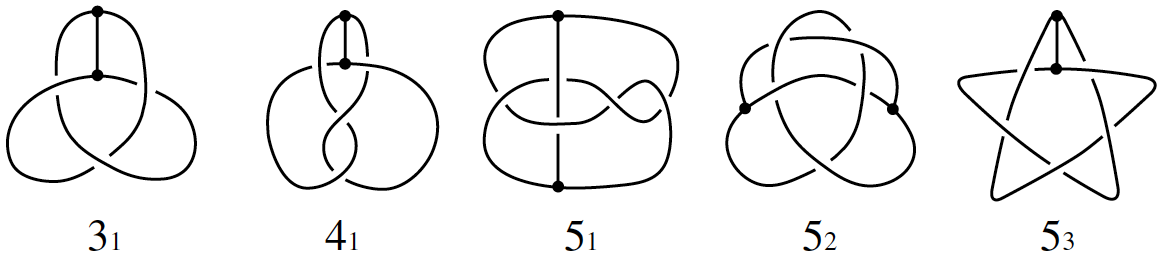
\includegraphics[width=.8\linewidth]{theta_exe.png}$$
	\end{itemize}
\end{frame}

\begin{frame}{Handcuff Graphs}
	\begin{itemize}
		\item \term{Handcuff graph} H is the graph which consists of two loops and an edge jointing the vertices of each loop.
		\item A \term{constituent link $H_{12}$}, is a subgraph of $H$
		that consists of two vertices $v_1$, $v_2$ and two edges $e_1$, $e_2$.

	\end{itemize}

	$$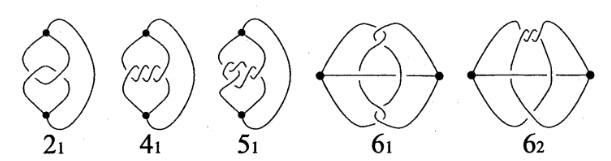
\includegraphics[width=.8\linewidth]{handcufflist.png}$$
\end{frame}

\begin{frame}{Reidemaister Moves for Theta-Curves and Handcuff Graphs}
	\medskip
	\begin{enumerate}
		\item[\mybf{I.}] \quad\raisebox{-15pt}{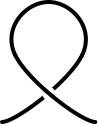
\includegraphics[width=36pt,height=36pt]{y101}} \quad $\longleftrightarrow$ \quad \raisebox{-15pt}{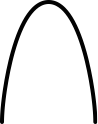
\includegraphics[width=36pt,height=36pt]{y103}} \quad $\longleftrightarrow$ \quad \raisebox{-15pt}{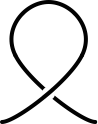
\includegraphics[width=36pt,height=36pt]{y102}}\medskip
		\item[\mybf{II.}] \quad\raisebox{-15pt}{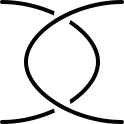
\includegraphics[width=36pt,height=36pt]{y111}} \quad $\longleftrightarrow$ \quad \raisebox{-15pt}{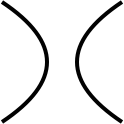
\includegraphics[width=36pt,height=36pt]{y93}} \quad $\longleftrightarrow$ \quad \raisebox{-15pt}{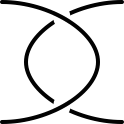
\includegraphics[width=36pt,height=36pt]{y112}}\medskip
		\item[\mybf{III.}] \quad\raisebox{-15pt}{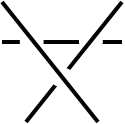
\includegraphics[width=36pt,height=36pt]{r31}} \quad $\longleftrightarrow$ \quad \raisebox{-15pt}{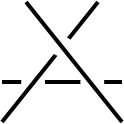
\includegraphics[width=36pt,height=36pt]{r32}} \qquad\qquad\raisebox{-15pt}{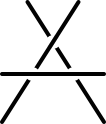
\includegraphics[width=36pt,height=36pt]{y121}} \quad $\longleftrightarrow$ \quad \raisebox{-15pt}{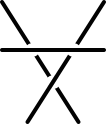
\includegraphics[width=36pt,height=36pt]{y122}}\medskip
		\item[\mybf{IV.}] \quad\raisebox{-15pt}{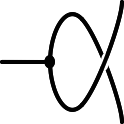
\includegraphics[width=36pt,height=36pt]{y141}} \quad $\longleftrightarrow$ \quad \raisebox{-15pt}{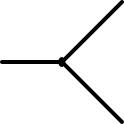
\includegraphics[width=36pt,height=36pt]{y143}} \quad $\longleftrightarrow$ \quad \raisebox{-15pt}{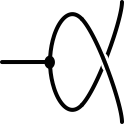
\includegraphics[width=36pt,height=36pt]{y142}}\medskip
		\item[\mybf{V.}] \quad\raisebox{-15pt}{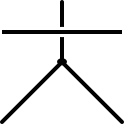
\includegraphics[width=36pt,height=36pt]{y131}} \quad $\longleftrightarrow$ \quad \raisebox{-15pt}{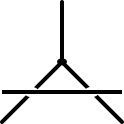
\includegraphics[width=36pt,height=36pt]{y132}} \qquad\qquad\raisebox{-15pt}{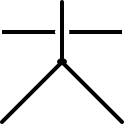
\includegraphics[width=36pt,height=36pt]{y133}} \quad $\longleftrightarrow$ \quad \raisebox{-15pt}{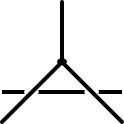
\includegraphics[width=36pt,height=36pt]{y134}}
	\end{enumerate}
\end{frame}

\begin{frame}{Arc Presentation}
    \begin{itemize}
        \item \term{Arc presentation} of a theta-curve or handcuff graph is an embedding of them.
        \item It is contained in the union of finitely many half planes (called \term{pages}).
        \item The embedding is with the common boundary line (called \term{axis}).
        \item Each vertex lies in the axis.
        \item Each page contains a properly embedded single arc.
        \item \term{Arc index}, is the minimal number of pages among all possible arc presentations of graph.
        \item This arc presentation with the minimal number of pages is \term{minimal arc presentation}.
    \end{itemize}
\end{frame}

\begin{frame}{Arc Presentation}
    \centering
    \begin{tabu}{X[c]X[c]X[c]}
        \raisebox{-1cm}{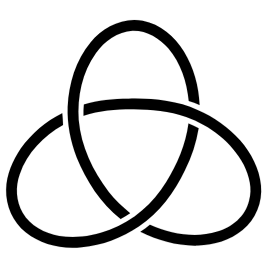
\includegraphics[height=1cm]{Trefoilimage.png}} &
        \raisebox{-1cm}{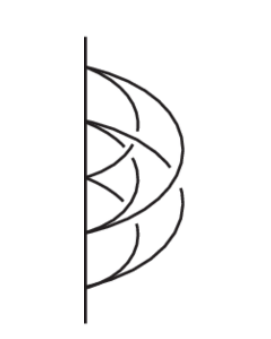
\includegraphics[height=1.75cm]{trefoil arc presentation.png}} &
        \raisebox{-1cm}{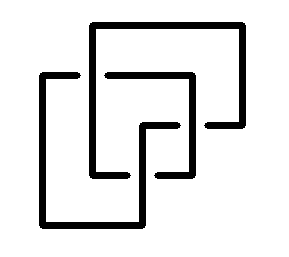
\includegraphics[height=1cm]{trefoil_grid.png}} \\
        Trefoil & Open Book & Grid Diagram
    \end{tabu}
    \centering
    \begin{tabu}{X[c]X[c]X[c]}
        \raisebox{-1cm}{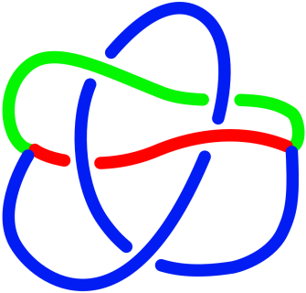
\includegraphics[height=1cm]{theta52.png}} &
        \raisebox{-1cm}{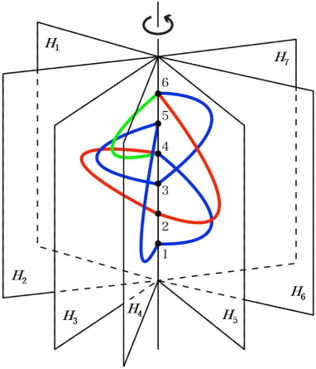
\includegraphics[height=1.75cm]{openbook.png}} &
        \raisebox{-1cm}{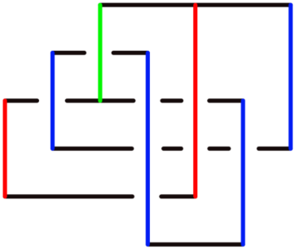
\includegraphics[height=1cm]{grid.png}} \\
        $\theta_{5,2}$ & Open Book & Grid Diagram
    \end{tabu}
    \centering
    \begin{tabu}{X[c]X[c]X[c]}
        \raisebox{-1cm}{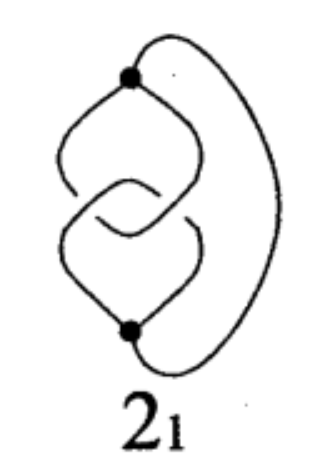
\includegraphics[height=2cm]{handcuff.png}} &
        \raisebox{-1cm}{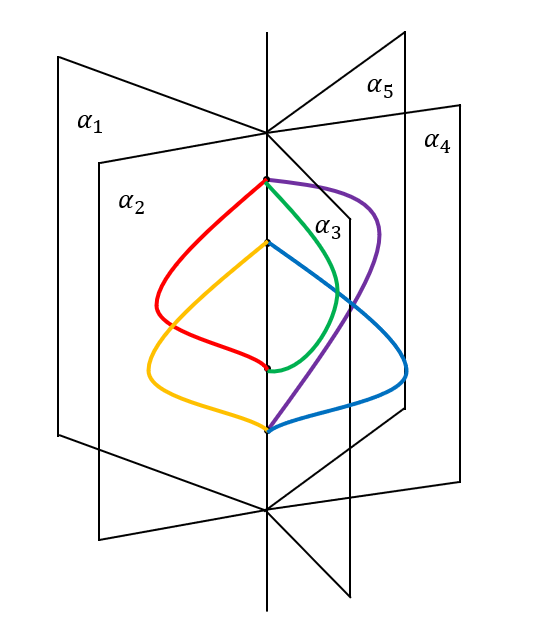
\includegraphics[height=1.75cm]{handcuff_openbook.png}} &
        \raisebox{-1cm}{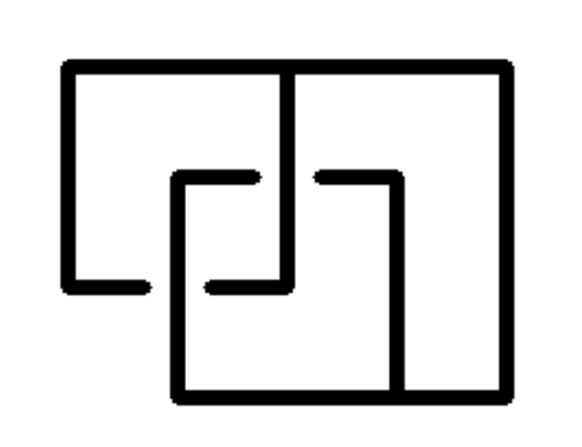
\includegraphics[height=1cm]{handcuff grid diagram.png}} \\
        $\Phi_{2,1}$ & Open Book & Grid Diagram
    \end{tabu}
\end{frame}


\begin{frame}{Grid Diagram}
	\begin{itemize}
        \item The \term{grid diagram} of theta-curve or handcuff graph is a diagram with only vertical strand and horizontal strands.
        \item (number of vertical strands) + 1 = (number of horizontal strands)
        \item At every crossing, the vertical strand crosses over the horizontal strand.
        \item No two horizontal strands are in the same row.
        \item No two vertical strands are in same strand.
    \end{itemize}
\end{frame}

\begin{frame}{Grid Diagram}
    \begin{itemize}
        \item A grid diagram gives rise to an arc presentation and vice versa.
    \end{itemize}
    \centering
    \begin{tabu}{X[c]X[c]}
        \raisebox{-1cm}{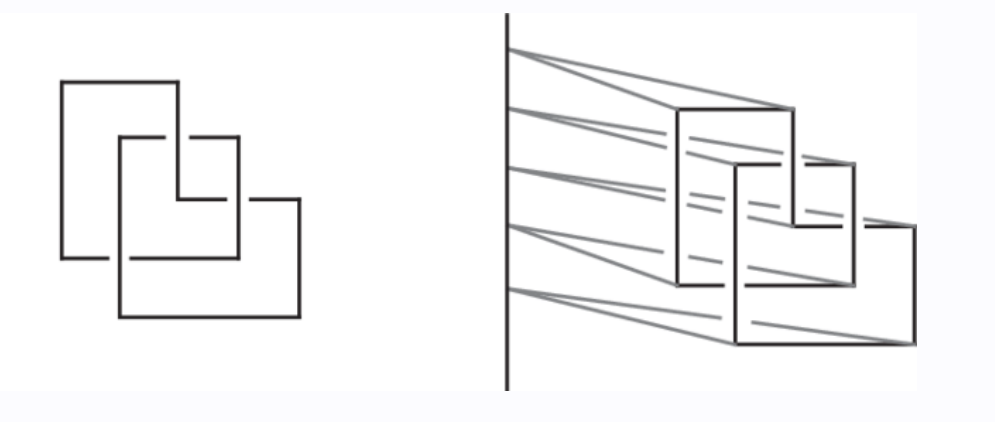
\includegraphics[height=4cm]{grid_diagram_1.png}} &
        \raisebox{-1cm}{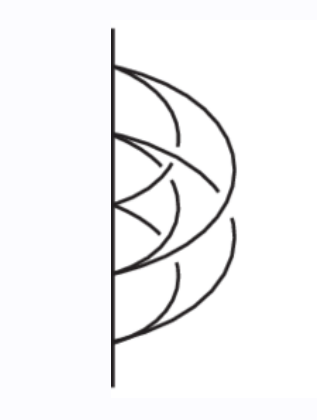
\includegraphics[height=4cm]{grid_diagram_2.png}} \\
    \end{tabu}
\end{frame}

\begin{frame}{Arc Presentation of the Theta-Curve and Handcuff Graph}
	\begin{thm}
    Every theta-curve and handcuff graph admit a grid diagram.
    \end{thm}
	\mypf
    \begin{center}
    \begin{tabu}{c c c}
        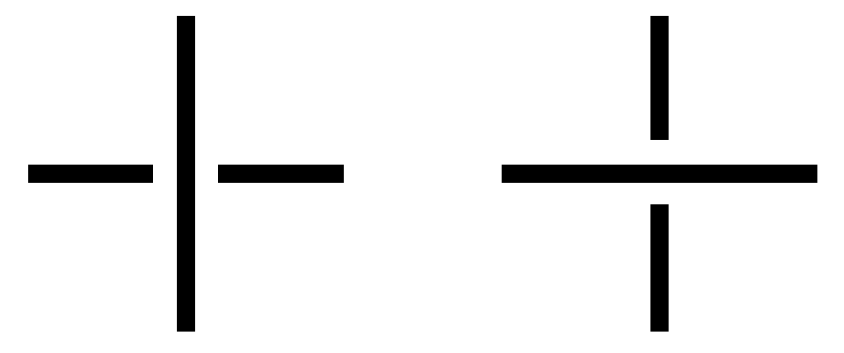
\includegraphics[width=0.2\linewidth]{figure/crossings.png} &
        \raisebox{0.5cm}{$\xmapsto{}$} &
        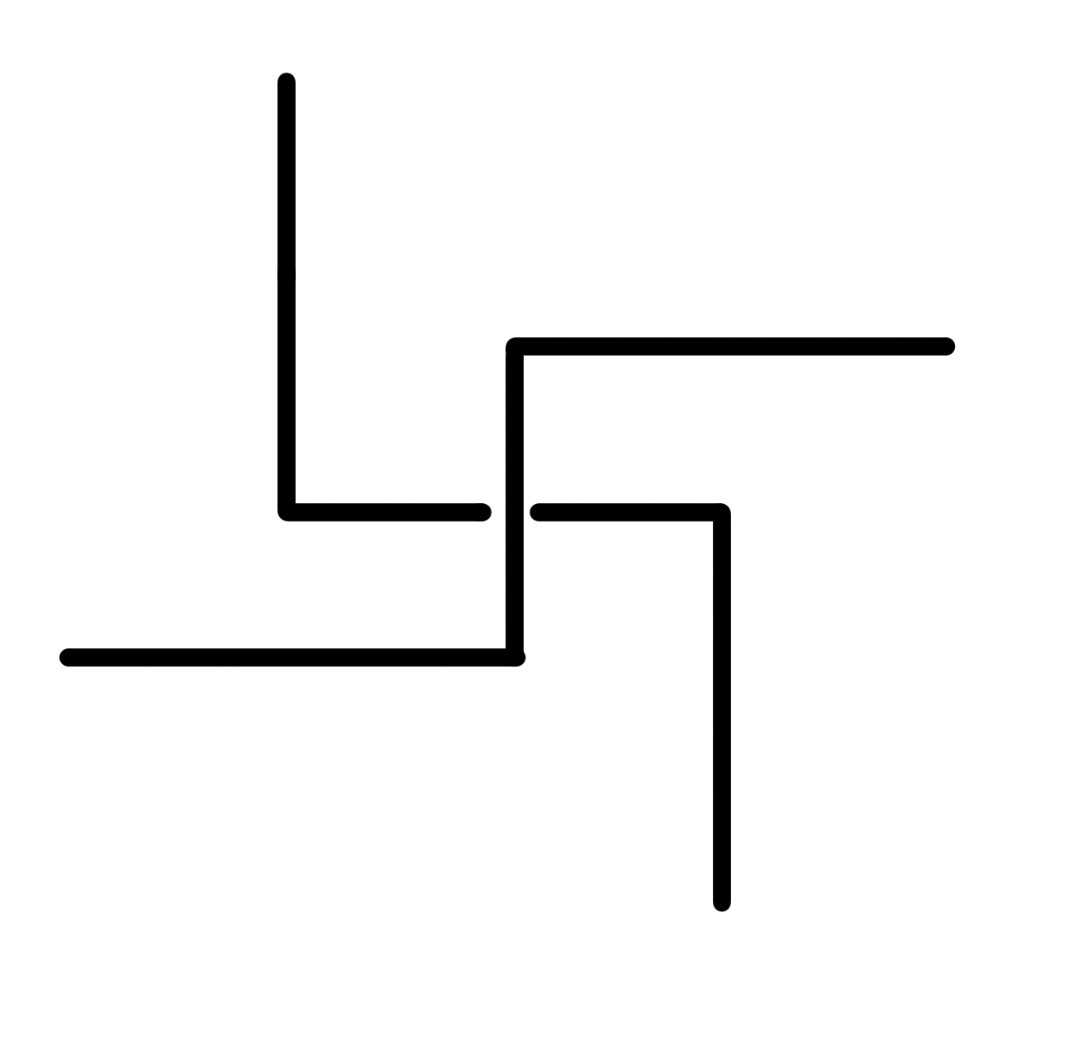
\includegraphics[width=0.1\linewidth]{changed_crossing.jpg}
    \end{tabu}
    \begin{tabu}{c}
        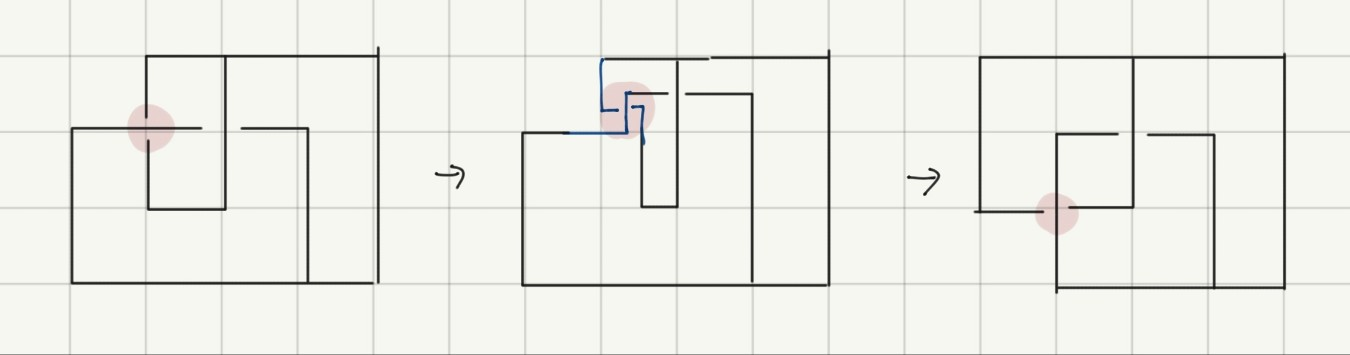
\includegraphics[width=0.5\linewidth]{crossing_change_example.jpg}
    \end{tabu}
    \end{center}
    \begin{corollary}
    Every theta-curve and handcuff graph admit a arc presentation.
    \end{corollary}
\end{frame}

\section{Classifying by Determinant}
\begin{frame}{THC-cromwell matrix}
	\begin{itemize}
		\item The \term{THC-cromwell matrix} is an expansion of cromwell matrix into $\theta$-curves and handcuff graphs
	\end{itemize}
	\vspace{1cm}
	\begin{tabu}{X[5c]X[c]X[5c]}
		\raisebox{-1.5cm}{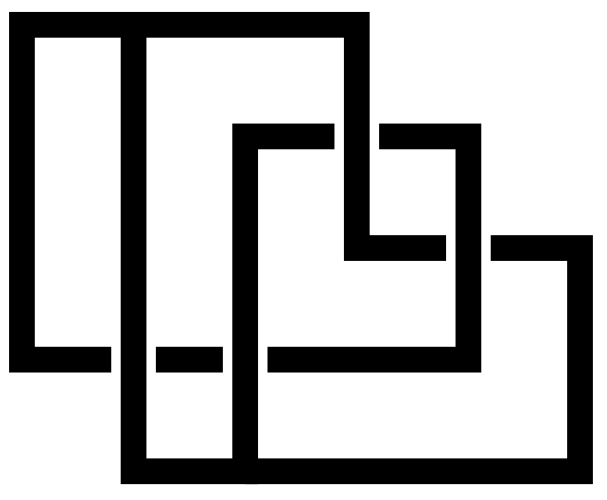
\includegraphics[height=3cm]{figure/excromwell.png}} &			
		$\longmapsto$ &
		\raisebox{-1.5cm}{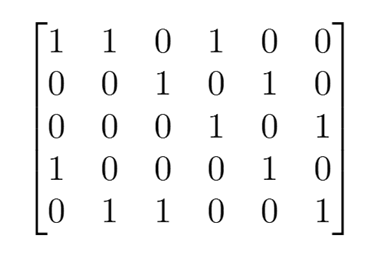
\includegraphics[height=3cm]{figure/cromwell.png}} &
	\end{tabu}
	
\end{frame}

\begin{frame}{Determinant of the cromwell matrices of Knot}
	\begin{thm}
		Let $K$ be any knot then its determinant of the cromwell matrix is $0$ or $\pm2$.
	\end{thm}
	\mypf
	\begin{tabu}{X[5c]X[2c]X[5c]X[c]X[2c]}
			\raisebox{-1.5cm}{\includegraphics[height=3cm]{trefoilimage.png}} &
			$\xmapsto{\text{grid diagram}}$ &
			\raisebox{-1.5cm}{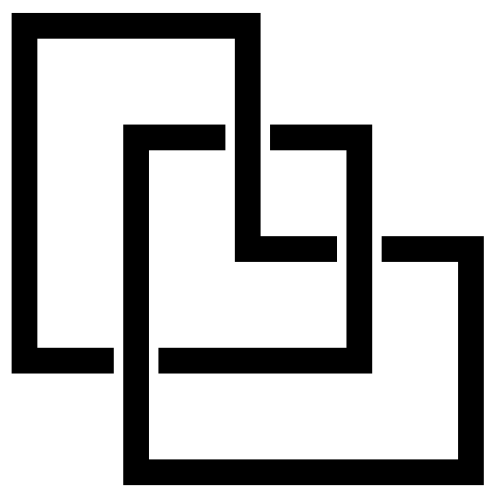
\includegraphics[height=3cm]{figure/gridtheta.png}} &
			$\xmapsto{THC-cromwell}$ &
	\end{tabu}
	\begin{tabu}{X[c]X[1.5c]X[5c]X[c]X[5c]}
			\raisebox{-1.5cm}{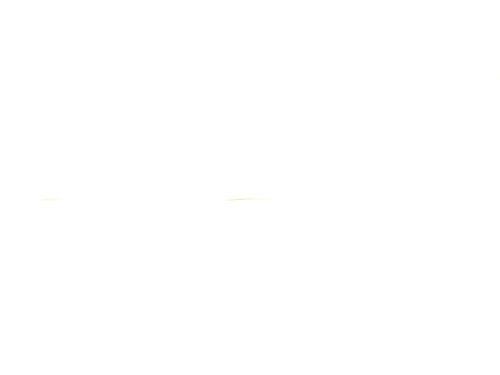
\includegraphics[height=3cm]{figure/white.png}} &
			$\xmapsto{THC-cromwell}$ &
			$\begin{bmatrix}
				\textcolor{red}{1} & 0 & \textcolor{red}{1} & 0 & 0\\
				0 & \textcolor{red}{1} & 0 & \textcolor{red}{1} & 0\\
				0 & 0 & \textcolor{red}{1} & 0 & \textcolor{red}{1}\\
				\textcolor{red}{1} & 0 & 0 & \textcolor{red}{1} & 0\\
				0 & \textcolor{red}{1} & 0 & 0 & \textcolor{red}{1}
			\end{bmatrix}$&
			$\xmapsto[operations]{row/column}$ &
			$\begin{bmatrix}
				\textcolor{red}{1} & \textcolor{red}{1} & 0 & 0 & 0\\
				0 & \textcolor{red}{1} & \textcolor{red}{1} & 0 & 0\\
				0 & 0 & \textcolor{red}{1} & \textcolor{red}{1} & 0\\
				0 & 0 & 0 & \textcolor{red}{1} & \textcolor{red}{1}\\
				\textcolor{red}{1} & 0 & 0 & 0 & \textcolor{red}{1}
			\end{bmatrix}$
	\end{tabu}
\end{frame}
\begin{frame}
	\begin{enumerate}
		\item[\mybf{CASE 1.}] \mybf{When $n$ is an even number.}
	\end{enumerate}
	%\vspace*{-10pt}
	\begin{tabu}{X[5c]X[c]X[5c]X[c]X[5c]}
		$\begin{bmatrix}
			\textcolor{red}{1} & \textcolor{red}{1} & 0 & 0 \\
			0 & \textcolor{red}{1} & \textcolor{red}{1} & 0\\
			0 & 0 & \textcolor{red}{1} & \textcolor{red}{1}\\
			\textcolor{red}{1} & 0 & 0 & \textcolor{red}{1}
		\end{bmatrix}$ &
		$\longmapsto$ &
		$\begin{bmatrix}
			\textcolor{red}{1} & \textcolor{red}{1} & 0 & 0 \\
			0 & \textcolor{red}{1} & \textcolor{red}{1} & 0\\
			0 & 0 & \textcolor{red}{1} & \textcolor{red}{1}\\
			\textcolor{PineGreen}{2} & \textcolor{PineGreen}{2} & \textcolor{PineGreen}{2} & \textcolor{PineGreen}{2}
		\end{bmatrix}$ &
		$\longmapsto$ &
		$\begin{bmatrix}
			\textcolor{red}{1} & \textcolor{red}{1} & 0 & 0 \\
			0 & \textcolor{red}{1} & \textcolor{red}{1} & 0\\
			0 & 0 & \textcolor{red}{1} & \textcolor{red}{1}\\
			\textcolor{Aquamarine}{0} & \textcolor{Aquamarine}{0} & \textcolor{Aquamarine}{0} & \textcolor{Aquamarine}{0}
		\end{bmatrix}$ &
	\end{tabu}
	So the determinant of $K$ is $0$.
	\begin{enumerate}
		\item[\mybf{CASE 2.}] \mybf{When $n$ is an odd number.}
	\end{enumerate}
	\begin{tabu}{X[5c]X[c]X[5c]X[c]X[5c]}
		$\begin{bmatrix}
			\textcolor{red}{1} & \textcolor{red}{1} & 0 & 0 & 0\\
			0 & \textcolor{red}{1} & \textcolor{red}{1} & 0 & 0\\
			0 & 0 & \textcolor{red}{1} & \textcolor{red}{1} & 0\\
			0 & 0 & 0 & \textcolor{red}{1} & \textcolor{red}{1}\\
			\textcolor{red}{1} & 0 & 0 & 0 & \textcolor{red}{1}
		\end{bmatrix}$ &
		$\longmapsto$ &
		$\begin{bmatrix}
			\textcolor{red}{1} & \textcolor{red}{1} & 0 & 0 & 0 \\
			0 & \textcolor{red}{1} & \textcolor{red}{1} & 0 & 0\\
			0 & 0 & \textcolor{red}{1} & \textcolor{red}{1} & 0\\
			0 & 0 & 0 & \textcolor{red}{1} & \textcolor{red}{1}\\
			\textcolor{PineGreen}{2} & \textcolor{PineGreen}{2} & \textcolor{PineGreen}{2} & \textcolor{PineGreen}{2} & \textcolor{PineGreen}{2}
		\end{bmatrix}$ &
		$\longmapsto$ &
		$\begin{bmatrix}
			\textcolor{red}{1} & \textcolor{red}{1} & 0 & 0 & 0 \\
			0 & \textcolor{red}{1} & \textcolor{red}{1} & 0 & 0\\
			0 & 0 & \textcolor{red}{1} & \textcolor{red}{1} & 0\\
			0 & 0 & 0 & \textcolor{red}{1} & \textcolor{red}{1}\\
			\textcolor{Aquamarine}{0} & \textcolor{Aquamarine}{0} & \textcolor{Aquamarine}{0} & \textcolor{Aquamarine}{0} & \textcolor{Cyan}{2}
		\end{bmatrix}$ &
	\end{tabu}
	So the determinant of $K$ is $\pm 2$.
	\hfill\qed
\end{frame}
\begin{frame}{H-deletion of THC-cromwell matricies}
	\begin{itemize}
		\item The \term{H-deletion} Matrix of the THC-cromwell
 		matrix G is $(n-1)\times(n-1)$ matrix\\ which deleted vertex-row and its two side-rows from the 
 		matrix G.
	\end{itemize}
	\vspace{1cm}
	\begin{tabu}{X[5c]X[c]X[5c]X[c]X[5c]}
			$\begin{bmatrix}
				\textcolor{red}{1} & 0 & \textcolor{red}{1} & 0 & 0 & \textcolor{red}{1}\\
				0 & \textcolor{red}{1} & 0 & \textcolor{red}{1} & 0 & 0\\
				0 & 0 & \textcolor{red}{1} & 0 & \textcolor{red}{1} & 0\\
				\textcolor{red}{1} & 0 & 0 & \textcolor{red}{1} & 0 & 0\\
				0 & \textcolor{red}{1} & 0 & 0 & \textcolor{red}{1} & \textcolor{red}{1}
			\end{bmatrix}$&
			$\longmapsto$ &
			$\begin{bmatrix}
			\textcolor{PineGreen}{1} & \textcolor{Aquamarine}{0} & \textcolor{PineGreen}{1} & \textcolor{Aquamarine}{0} & \textcolor{Aquamarine}{0} & \textcolor{PineGreen}{1}\\
				\textcolor{Aquamarine}{0} & \textcolor{red}{1} & 0 & \textcolor{red}{1} & 0 & \textcolor{Aquamarine}{0}\\
				\textcolor{Aquamarine}{0} & 0 & \textcolor{red}{1} & 0 & \textcolor{red}{1} & \textcolor{Aquamarine}{0}\\
				\textcolor{PineGreen}{1} & 0 & 0 & \textcolor{red}{1} & 0 & \textcolor{Aquamarine}{0}\\
				\textcolor{Aquamarine}{0} & \textcolor{red}{1} & 0 & 0 & \textcolor{red}{1} & \textcolor{PineGreen}{1}
			\end{bmatrix}$&
			$\longmapsto$ &
			$\begin{bmatrix}
				\textcolor{red}{1} & 0 & \textcolor{red}{1} & 0\\
				0 & \textcolor{red}{1} & 0 & \textcolor{red}{1}\\
				0 & 0 & \textcolor{red}{1} & 0\\
				\textcolor{red}{1} & 0 & 0 & \textcolor{red}{1}
			\end{bmatrix}$
	\end{tabu}
	
\end{frame}

\begin{frame}{Determinant of the THC-cromwell matrices}
	\begin{thm}
		Let $M$ be any THC-cromwell matrice of $\theta$-curve or handcuff graph. \\
		\begin{itemize}
			\item det($M$) = $\pm1$ $\iff$ $M$ represents $\theta$-curve
			\item det($M$) = $0$ or $\pm2$ $\iff$ $M$ represents handcuff graph
		\end{itemize}
		*det($M$) = determinant of H-deletion matrix of $M$
	\end{thm}
	\mypf
	\begin{tabu}{X[5c]X[c]X[5c]X[c]X[5c]}
			$\begin{bmatrix}
			\textcolor{RoyalBlue}{1} & 0 & \textcolor{RoyalBlue}{1} & 0 & \textcolor{RoyalBlue}{1} & 0 & 0\\
			0 & \textcolor{RoyalBlue}{1} & 0 & 0 & 0 & 0 & \textcolor{RoyalBlue}{1}\\
			\textcolor{RoyalBlue}{1} & 0 & 0 & \textcolor{RoyalBlue}{1} & 0 & 0 & 0\\
			0 & 0 & \textcolor{RoyalBlue}{1} & 0 & 0 & \textcolor{RoyalBlue}{1} & 0\\ 
			0 & 0 & 0 & 0 & \textcolor{RoyalBlue}{1} & 0 & \textcolor{RoyalBlue}{1}\\
			0 & \textcolor{RoyalBlue}{1} & 0 & \textcolor{RoyalBlue}{1} & 0 & \textcolor{RoyalBlue}{1} & 0\\
			\end{bmatrix}$&
			$\longmapsto$ &
			\raisebox{-1.5cm}{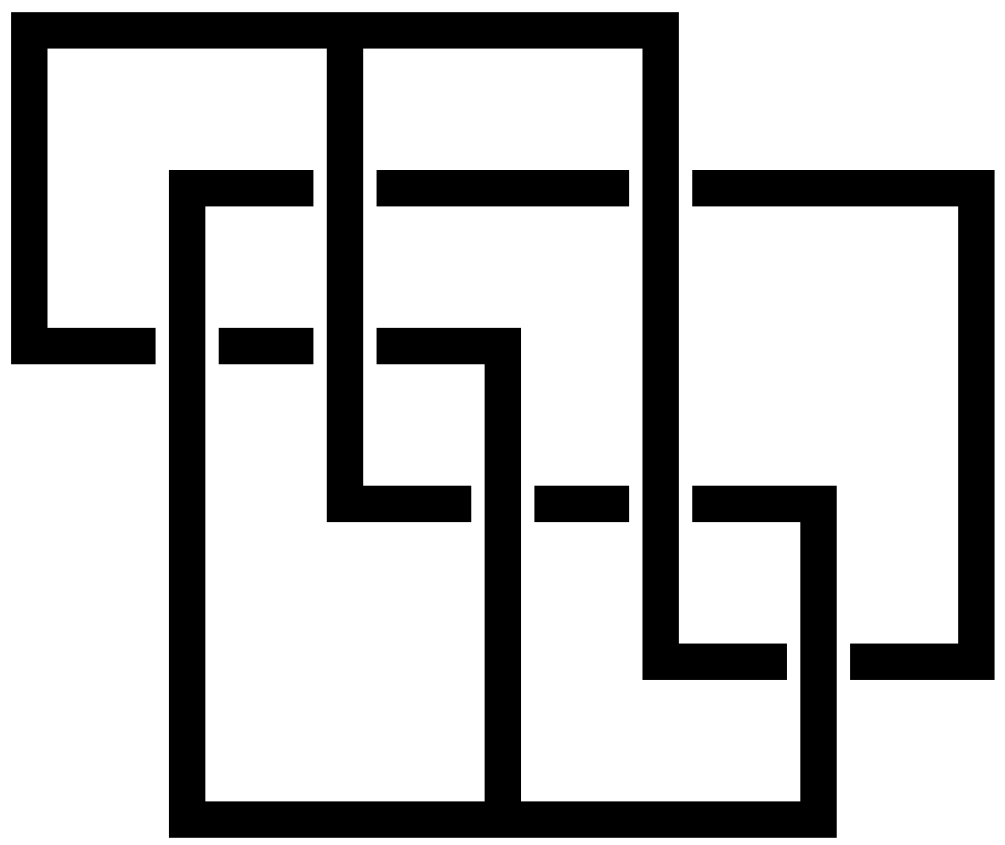
\includegraphics[height=3cm]{figure/exT-shape.png}} &
			$\longmapsto$ &
			\raisebox{-1.5cm}{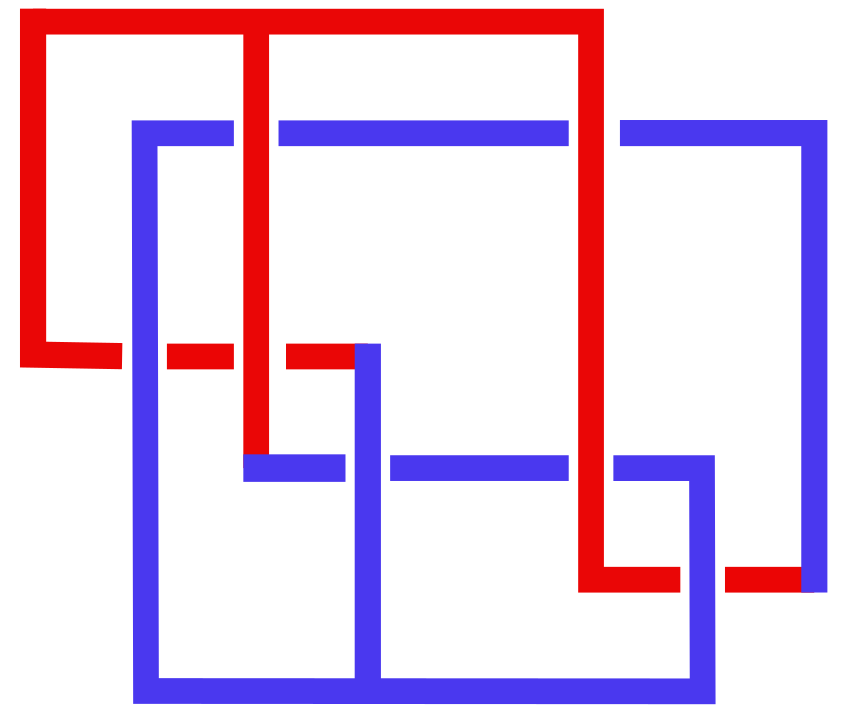
\includegraphics[height=3cm]{figure/T-shape.png}} 
	\end{tabu}
\end{frame}

\begin{frame}
	\begin{enumerate}
		\item[\mybf{CASE 1.}] \mybf{When $M$ represents $\theta$-curve}
	\end{enumerate}
	\mybfff{\circled{i} Line-shape} \\
	\begin{tabu}{X[5c]X[c]X[5c]X[c]X[5c]}
			\raisebox{-1.5cm}{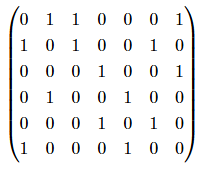
\includegraphics[height=3cm]{figure/L-shape.png}}&
			$\longmapsto$ &
			\raisebox{-1.5cm}{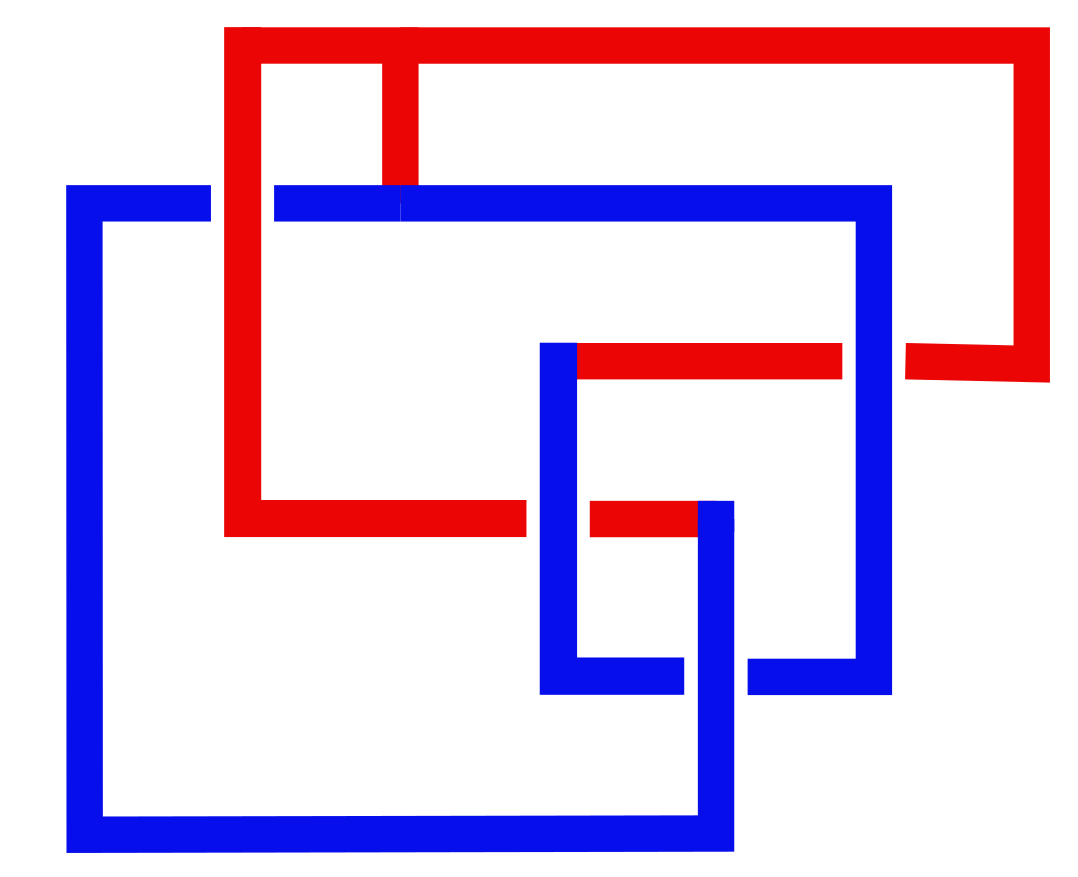
\includegraphics[height=3cm]{figure/Line-shape.png}} &
			$\xmapsto{H-deletion}$ &
			$\begin{bmatrix}
			\textcolor{RoyalBlue}{1} & \textcolor{RoyalBlue}{1} & 0 & 0 & \textcolor{RoyalBlue}{1} \\
			0 & 0 & \textcolor{RoyalBlue}{1} & 0 & 0\\
			0 & 0 & 0 & \textcolor{RoyalBlue}{1} & 0\\
			0 & 0 & \textcolor{RoyalBlue}{1} & 0 & \textcolor{RoyalBlue}{1} \\
			\textcolor{RoyalBlue}{1} & 0 & 0 & \textcolor{RoyalBlue}{1} & 0\\
		\end{bmatrix}$ &
	\end{tabu} \\
	and simplify with
	\begin{tabu}{X[c]X[5c]X[c]X[5c]}
		$\xmapsto[operations]{row/column}$ &
		$\begin{bmatrix}
			\textcolor{RoyalBlue}{1} & 0 & 0 & 0 & 0\\
			\textcolor{RoyalBlue}{1} & \textcolor{RoyalBlue}{1} & 0 & 0 & 0\\
			0 & \textcolor{RoyalBlue}{1} & \textcolor{RoyalBlue}{1} & 0 & \textcolor{RoyalBlue}{1}\\
			0 & 0 & \textcolor{RoyalBlue}{1} & \textcolor{RoyalBlue}{1} & 0\\
			0 & 0 & 0 & \textcolor{RoyalBlue}{1} & 0\\
		\end{bmatrix}$ &
		$\xmapsto{subtracting}$ &
		$\begin{bmatrix}
			\textcolor{red}{1} & 0& 0 & 0 & 0 \\
			0 & \textcolor{red}{1} & 0 & 0 & 0\\
			0 & 0 & \textcolor{red}{1} & 0 & \textcolor{red}{1}\\
			0 & 0 & 0 & \textcolor{red}{1} & \textcolor{red}{-1}\\
			0 & 0 & 0 & 0 & \textcolor{red}{1}\\
		\end{bmatrix}$ 
	\end{tabu}
	So det($M$) = $\pm1$
\end{frame}

\begin{frame}
	\begin{enumerate}
		\item[\mybf{CASE 1.}] \mybf{When $M$ represents $\theta$-curve}
	\end{enumerate}
	\mybfff{\circled{ii} T-shape} \\
	\begin{tabu}{X[5c]X[c]X[5c]X[c]X[5c]}
			$\begin{bmatrix}
			\textcolor{RoyalBlue}{1} & 0 & \textcolor{RoyalBlue}{1} & 0 & \textcolor{RoyalBlue}{1} & 0 & 0\\
			0 & \textcolor{RoyalBlue}{1} & 0 & 0 & 0 & 0 & \textcolor{RoyalBlue}{1}\\
			\textcolor{RoyalBlue}{1} & 0 & 0 & \textcolor{RoyalBlue}{1} & 0 & 0 & 0\\
			0 & 0 & \textcolor{RoyalBlue}{1} & 0 & 0 & \textcolor{RoyalBlue}{1} & 0\\ 
			0 & 0 & 0 & 0 & \textcolor{RoyalBlue}{1} & 0 & \textcolor{RoyalBlue}{1}\\
			0 & \textcolor{RoyalBlue}{1} & 0 & \textcolor{RoyalBlue}{1} & 0 & \textcolor{RoyalBlue}{1} & 0\\
			\end{bmatrix}$&
			$\longmapsto$ &
			\raisebox{-1.5cm}{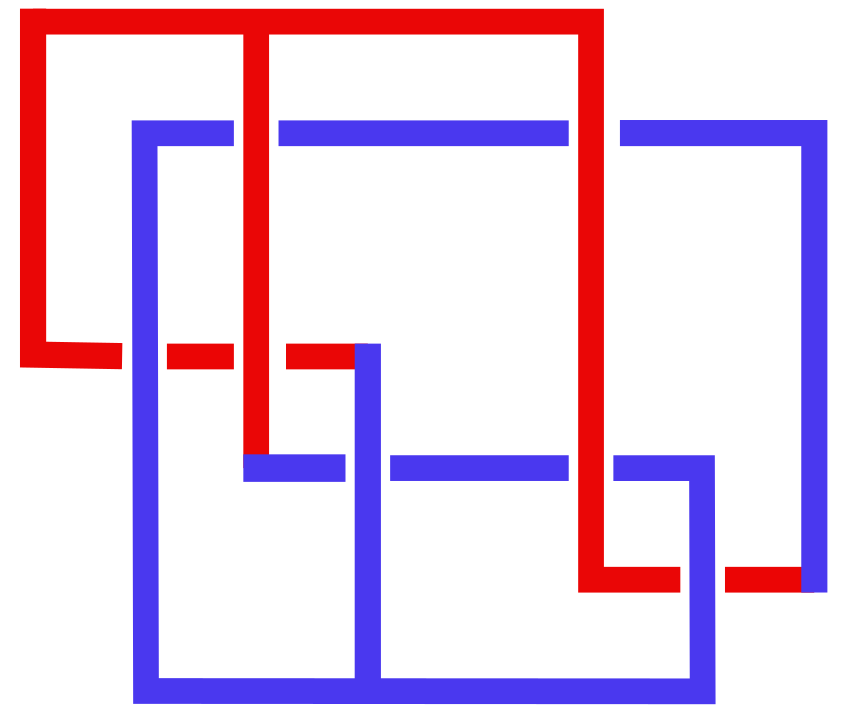
\includegraphics[height=3cm]{figure/T-shape.png}} &
			$\xmapsto{H-deletion}$ &
			$\begin{bmatrix}
			\textcolor{RoyalBlue}{1} & 0 & 0 & 0 & \textcolor{RoyalBlue}{1} \\
			0 & 0 & \textcolor{RoyalBlue}{1} & 0 & 0\\
			0 & \textcolor{RoyalBlue}{1} & 0 & \textcolor{RoyalBlue}{1} & 0\\
			0 & 0 & 0 & 0 & \textcolor{RoyalBlue}{1} \\
			\textcolor{RoyalBlue}{1} & 0 & \textcolor{RoyalBlue}{1} & \textcolor{RoyalBlue}{1} & 0\\
		\end{bmatrix}$ &
	\end{tabu} \\
	and simplify with
	\begin{tabu}{X[c]X[5c]X[c]X[5c]}
		$\xmapsto[operations]{row/column}$ &
		$\begin{bmatrix}
			\textcolor{RoyalBlue}{1} & 0 & 0 & 0 & 0\\
			\textcolor{RoyalBlue}{1} & \textcolor{RoyalBlue}{1} & 0 & \textcolor{RoyalBlue}{1} & 0\\
			0 & \textcolor{RoyalBlue}{1} & \textcolor{RoyalBlue}{1} & 0 & 0\\
			0 & 0 & 0 & \textcolor{RoyalBlue}{1} & \textcolor{RoyalBlue}{1}\\
			0 & 0 & 0 & 0 & \textcolor{RoyalBlue}{1}\\
		\end{bmatrix}$ &
		$\xmapsto{regioning}$ &
		\raisebox{-1.5cm}{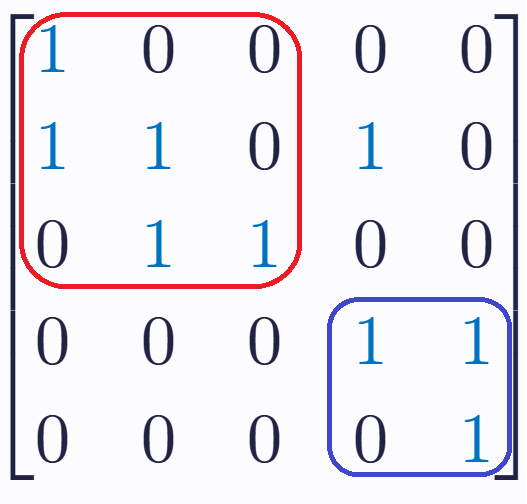
\includegraphics[height=3cm]{figure/regioning.png}}
	\end{tabu}
	So det($M$) = $\pm1$
\end{frame}


\begin{frame}
	\begin{enumerate}
		\item[\mybf{CASE 2.}] \mybf{When $M$ represents handcuff graph}
	\end{enumerate}
	\begin{tabu}{X[6c]X[c]X[4c]X[c]X[4c]}
			$\begin{bmatrix}
			0 & 0 & \textcolor{RoyalBlue}{1} & 0 & 0 & 0 & 0 & \textcolor{RoyalBlue}{1}\\
			0 & 0 & 0 & 0 & 0 & 0 & \textcolor{RoyalBlue}{1} & \textcolor{RoyalBlue}{1}\\
			\textcolor{RoyalBlue}{1} & 0 & \textcolor{RoyalBlue}{1} & 0 & 0 & 0 & 0 & 0\\
			\textcolor{RoyalBlue}{1} & 0 & 0 & 0 & \textcolor{RoyalBlue}{1} & 0 & \textcolor{RoyalBlue}{1} & 0\\
			0 & 0 & 0 & \textcolor{RoyalBlue}{1} & \textcolor{RoyalBlue}{1} & 0 & 0 & 0\\
			0 & \textcolor{RoyalBlue}{1} & 0 & \textcolor{RoyalBlue}{1} & 0 & \textcolor{RoyalBlue}{1} & 0 & 0\\
			0 & \textcolor{RoyalBlue}{1} & 0 & 0 & 0 & \textcolor{RoyalBlue}{1} & 0 & 0\\
			\end{bmatrix}$&
			$\longmapsto$ &
			\raisebox{-1.5cm}{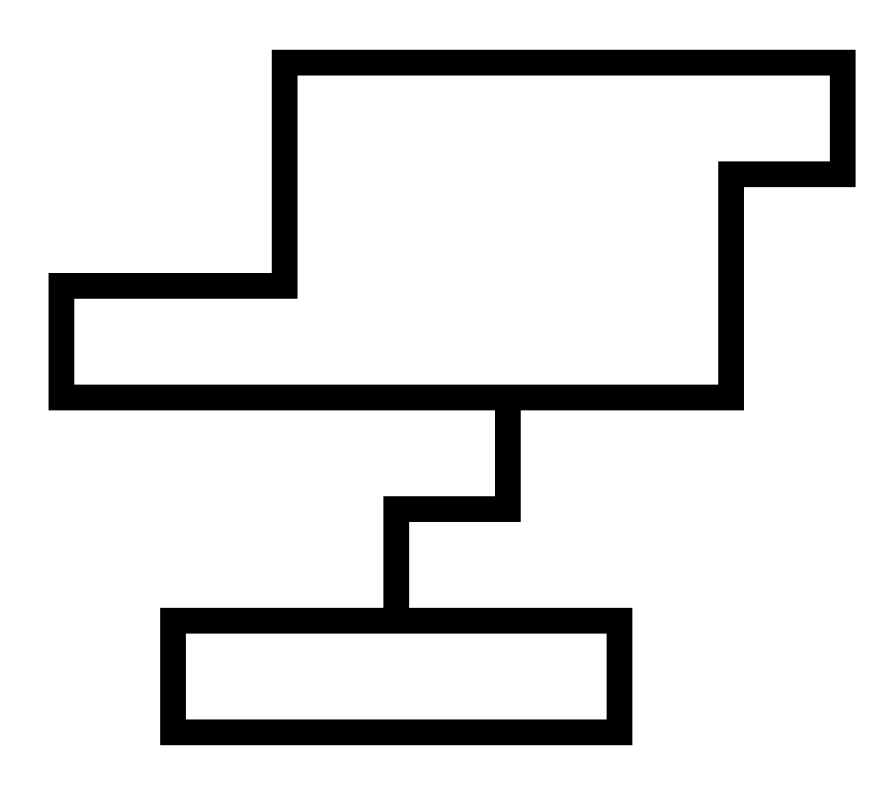
\includegraphics[height=3cm]{figure/blackgrid.png}} &
			$\longmapsto$ &
			\raisebox{-1.5cm}{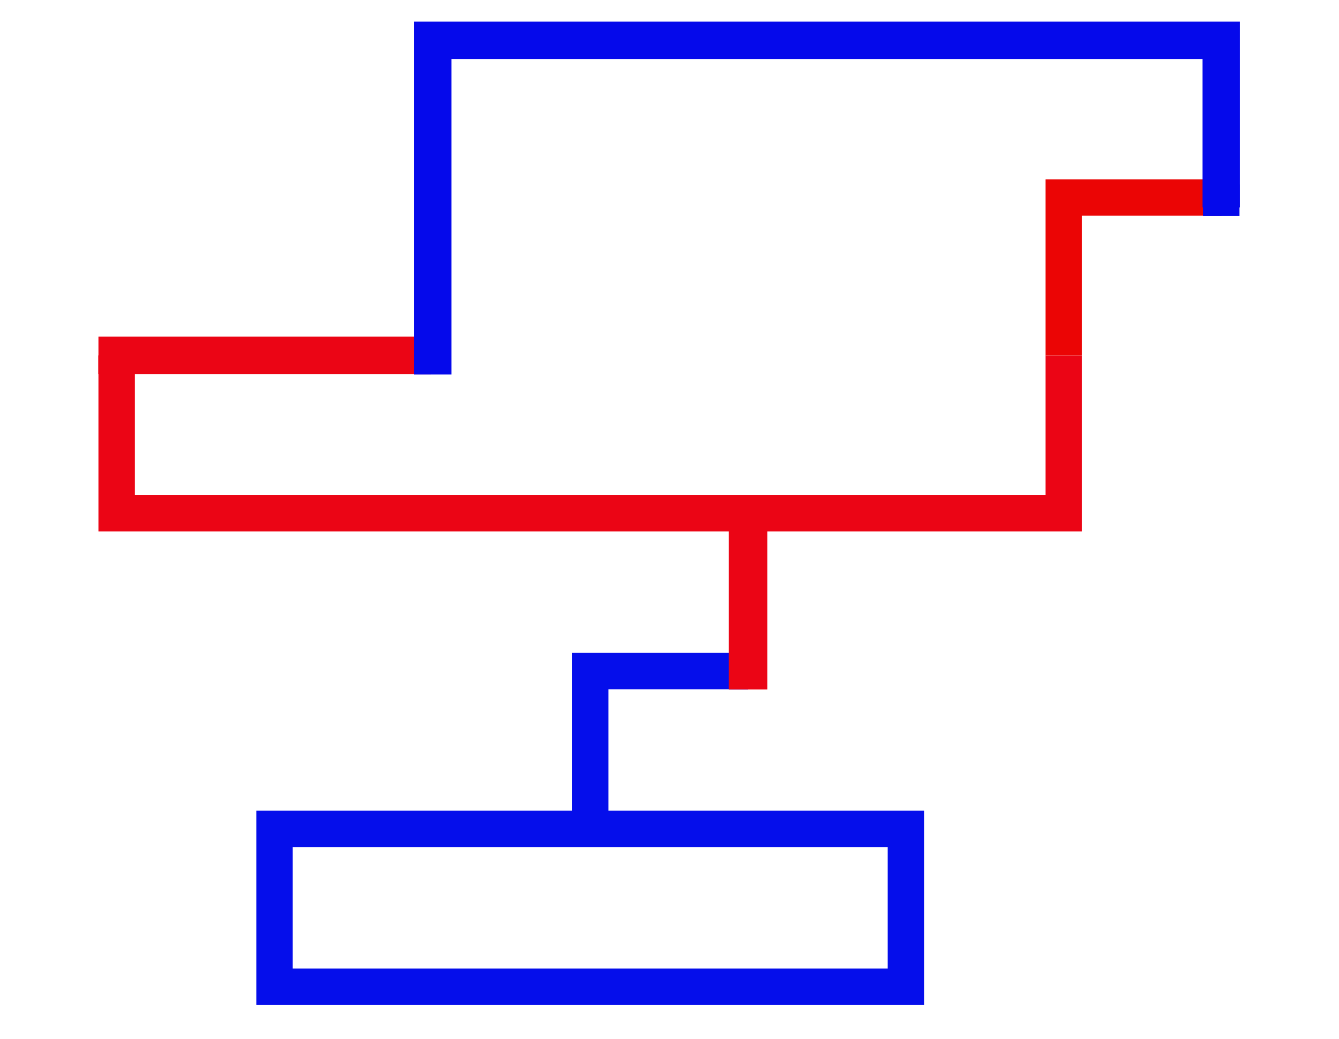
\includegraphics[height=3cm]{figure/T-loop.png}} 
	\end{tabu}
\end{frame}
\begin{frame}
	\begin{enumerate}
		\item[\mybf{CASE 2.}] \mybf{When $M$ represents handcuff graph}
	\end{enumerate}
	\mybfff{T-loop} \\
	\begin{tabu}{X[6c]X[c]X[4c]X[2c]X[2c]}
			$\begin{bmatrix}
			0 & 0 & \textcolor{RoyalBlue}{1} & 0 & 0 & 0 & 0 & \textcolor{RoyalBlue}{1}\\
			0 & 0 & 0 & 0 & 0 & 0 & \textcolor{RoyalBlue}{1} & \textcolor{RoyalBlue}{1}\\
			\textcolor{RoyalBlue}{1} & 0 & \textcolor{RoyalBlue}{1} & 0 & 0 & 0 & 0 & 0\\
			\textcolor{RoyalBlue}{1} & 0 & 0 & 0 & \textcolor{RoyalBlue}{1} & 0 & \textcolor{RoyalBlue}{1} & 0\\
			0 & 0 & 0 & \textcolor{RoyalBlue}{1} & \textcolor{RoyalBlue}{1} & 0 & 0 & 0\\
			0 & \textcolor{RoyalBlue}{1} & 0 & \textcolor{RoyalBlue}{1} & 0 & \textcolor{RoyalBlue}{1} & 0 & 0\\
			0 & \textcolor{RoyalBlue}{1} & 0 & 0 & 0 & \textcolor{RoyalBlue}{1} & 0 & 0\\
			\end{bmatrix}$&
			$\longmapsto$ &
			\raisebox{-1.5cm}{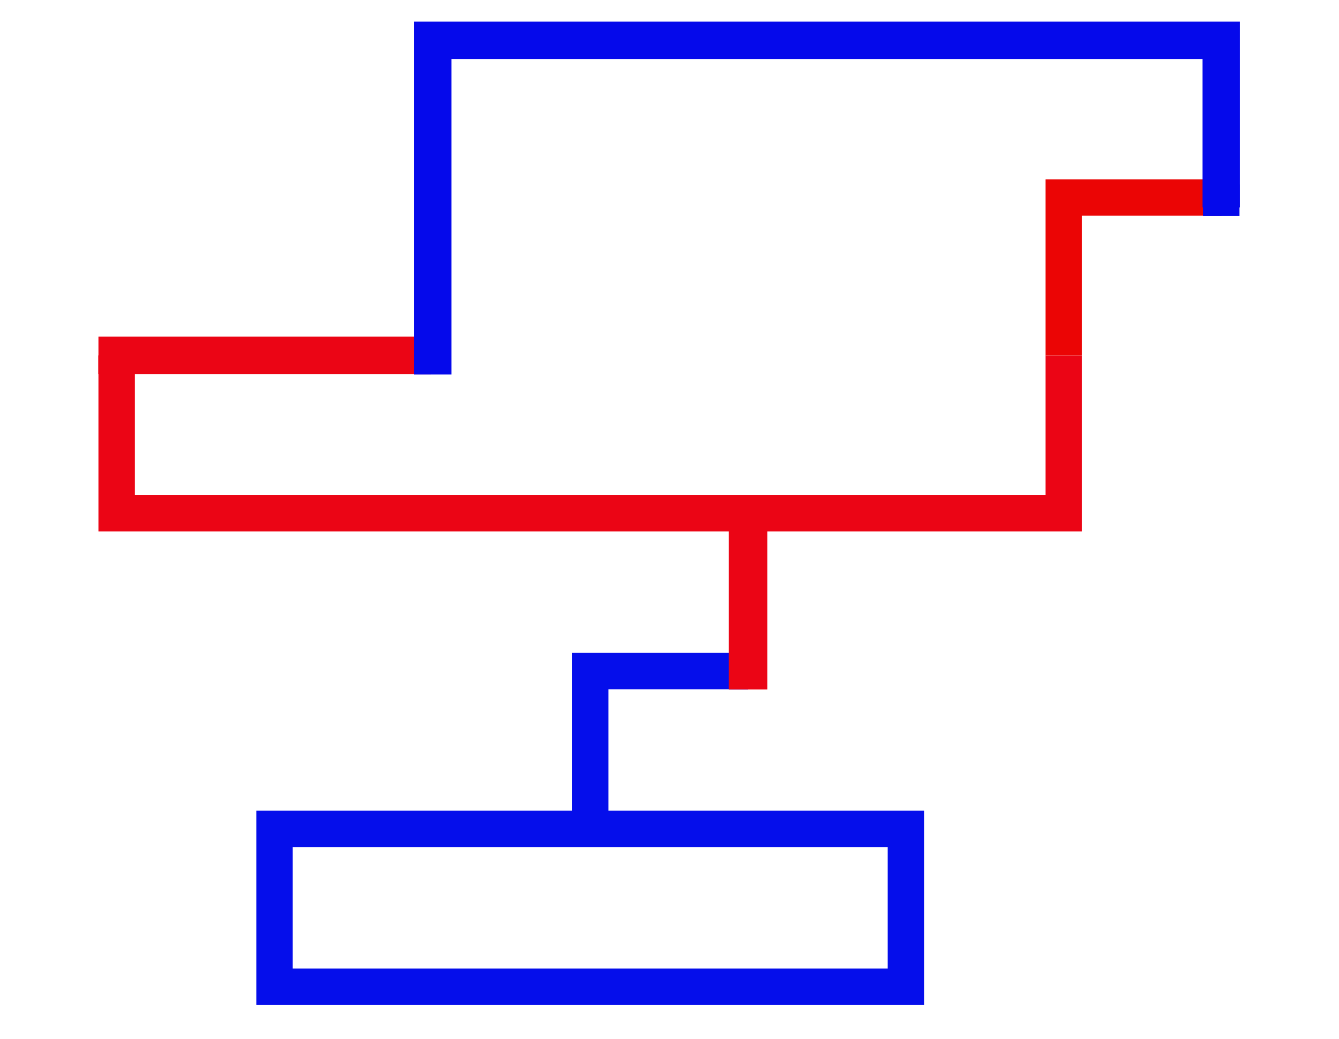
\includegraphics[height=3cm]{figure/T-loop.png}} &
			$\xmapsto{H-deletion}$ &
			$\begin{bmatrix}
			0 & \textcolor{RoyalBlue}{1} & 0 \\
			\textcolor{RoyalBlue}{1} & \textcolor{RoyalBlue}{1} & \textcolor{RoyalBlue}{1} \\
			 \textcolor{RoyalBlue}{1}& 0 & \textcolor{RoyalBlue}{1} \\
		\end{bmatrix}$ &
	\end{tabu} \\
	and simplify with
	\begin{tabu}{X[c]X[2c]X[c]X[3c]}
		$\xmapsto[operations]{row/column}$ &
		$\begin{bmatrix}
			\textcolor{RoyalBlue}{1} & \textcolor{RoyalBlue}{1} & 0 \\
			\textcolor{RoyalBlue}{1} & \textcolor{RoyalBlue}{1} & \textcolor{RoyalBlue}{1} \\
			0 & 0 & \textcolor{RoyalBlue}{1} \\
		\end{bmatrix}$ &
		$\xmapsto{seperating}$ &
		$\begin{bmatrix}
			\textcolor{RoyalBlue}{Knot} & * \\
			O & \textcolor{RoyalBlue}{Line-shape} \\
		\end{bmatrix}$ &
	\end{tabu}
	So det($M$) = 0 or $\pm2$
\end{frame}
\begin{frame}
	\begin{enumerate}
		\item[\mybf{CASE 2.}] \mybf{When $M$ represents handcuff graph}
	\end{enumerate}
	\mybfff{\circled{i} T-loop \& Line-shape}\\
	\begin{tabu}{X[6c]X[c]X[4c]X[2c]X[3c]}
			$\begin{bmatrix}
			0 & 0 & \textcolor{RoyalBlue}{1} & 0 & 0 & 0 & 0 & \textcolor{RoyalBlue}{1}\\
			0 & 0 & 0 & 0 & 0 & 0 & \textcolor{RoyalBlue}{1} & \textcolor{RoyalBlue}{1}\\
			\textcolor{RoyalBlue}{1} & 0 & \textcolor{RoyalBlue}{1} & 0 & 0 & 0 & 0 & 0\\
			\textcolor{RoyalBlue}{1} & 0 & 0 & 0 & \textcolor{RoyalBlue}{1} & 0 & \textcolor{RoyalBlue}{1} & 0\\
			0 & 0 & 0 & \textcolor{RoyalBlue}{1} & \textcolor{RoyalBlue}{1} & 0 & 0 & 0\\
			0 & \textcolor{RoyalBlue}{1} & 0 & \textcolor{RoyalBlue}{1} & 0 & \textcolor{RoyalBlue}{1} & 0 & 0\\
			0 & \textcolor{RoyalBlue}{1} & 0 & 0 & 0 & \textcolor{RoyalBlue}{1} & 0 & 0\\
			\end{bmatrix}$&
			$\longmapsto$ &
			\raisebox{-1.5cm}{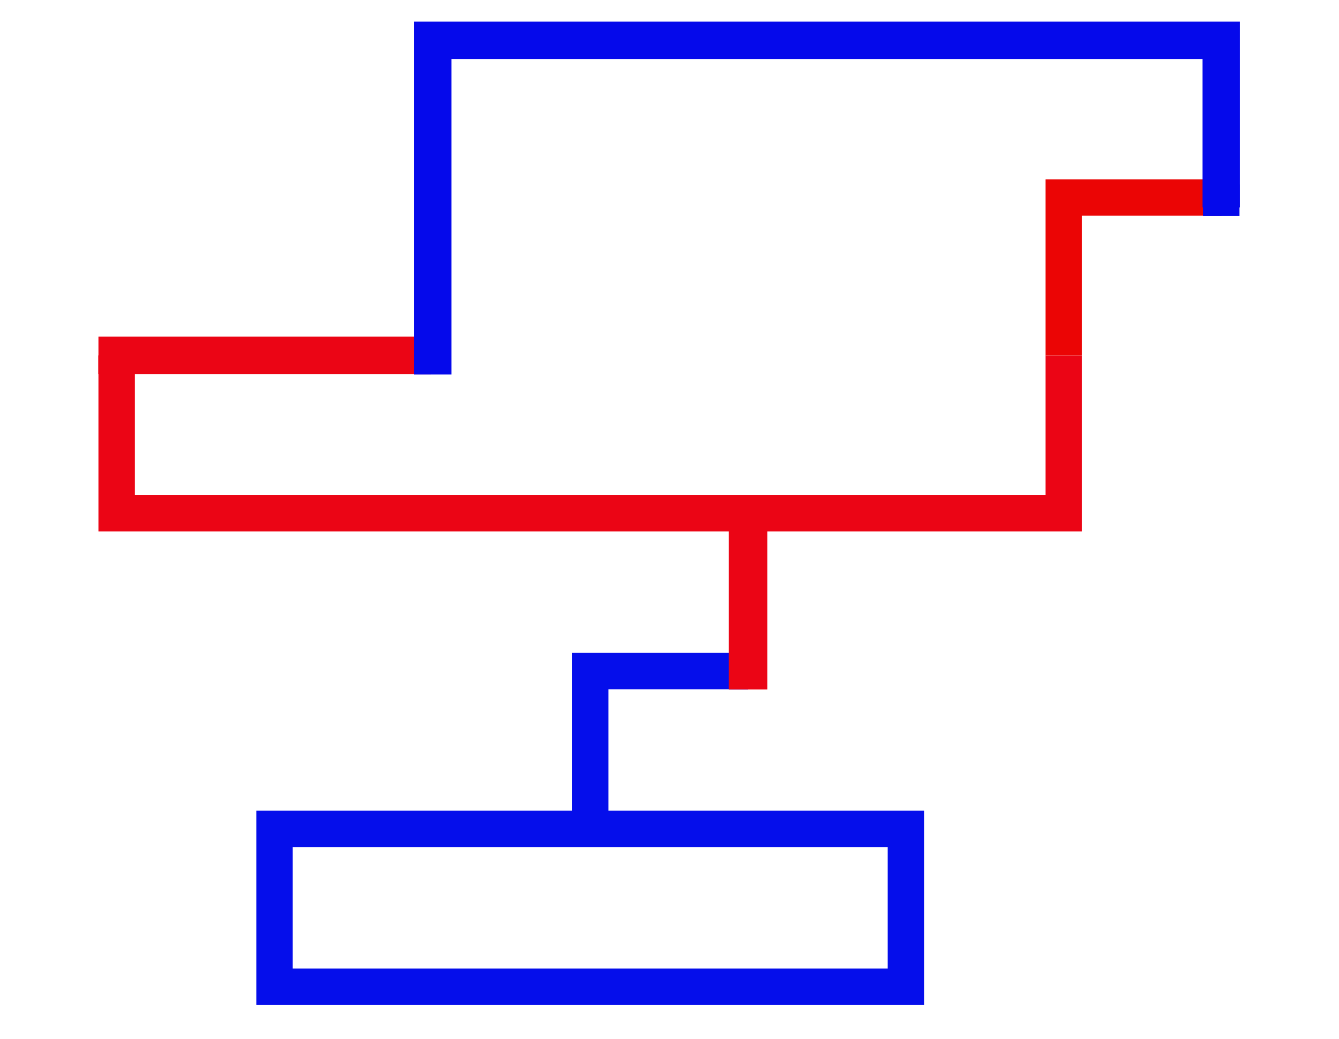
\includegraphics[height=3cm]{figure/T-loop.png}} &
			$\xmapsto{H-deletion}$ &
			$\begin{bmatrix}
			0 & \textcolor{RoyalBlue}{1} & 0 & 0 & 0 & \textcolor{RoyalBlue}{1}\\
			0 & 0 & 0 & 0 & 0 & \textcolor{RoyalBlue}{1}\\
			0 & \textcolor{RoyalBlue}{1} & 0 & 0 & 0 & 0\\
			0 & 0 & \textcolor{RoyalBlue}{1} & \textcolor{RoyalBlue}{1} & 0 & 0\\
			\textcolor{RoyalBlue}{1} & 0 & \textcolor{RoyalBlue}{1} & 0 & \textcolor{RoyalBlue}{1} & 0\\
			\textcolor{RoyalBlue}{1} & 0 & 0 & 0 & \textcolor{RoyalBlue}{1} & 0\\
			\end{bmatrix}$&
	\end{tabu} \\
	and simplify with
	\begin{tabu}{X[c]X[3c]X[c]X[4c]}
		$\xmapsto{operations}$ &
		$\begin{bmatrix}
			\textcolor{RoyalBlue}{T-loop} & *\\
			0 & \textcolor{RoyalBlue}{Line-shape} \\
		\end{bmatrix}$&
		$\xmapsto{seperating}$ &
		$\begin{bmatrix}
			\textcolor{RoyalBlue}{Knot} & * & * \\
			0 & \textcolor{RoyalBlue}{Line-shape} & * \\
			0 & 0 & \textcolor{RoyalBlue}{Line-shape} \\
		\end{bmatrix}$ &
	\end{tabu}
	So det($M$) = 0 or $\pm2$
\end{frame}
\begin{frame}
	\begin{enumerate}
		\item[\mybf{CASE 2.}] \mybf{When $M$ represents handcuff graph}
	\end{enumerate}
	\mybfff{\circled{ii} Knot \& Line-shape}\\
	\begin{tabu}{X[3c]X[2c]X[3c]X[2c]X[3c]}
			cromwell matrix&
			$\xmapsto{H-deletion}$ &
			H-deletion matrix&
			$\xmapsto[operations]{seperating}$ &
		$\begin{bmatrix}
			\textcolor{RoyalBlue}{Knot} & * \\
			O & \textcolor{RoyalBlue}{Line-shape} \\
		\end{bmatrix}$ &
	\end{tabu} \\
	So det($M$) = 0 or $\pm2$
\end{frame}
%\include{L Bound.tex}

\begin{frame}[standout,plain]
	\TINY
	\bibliographystyle{apalike}
	\nocite{*}
	\bibliography{KnSG2024}
\end{frame}

\end{document}